\documentclass{article}

\usepackage{amsmath}
\usepackage{graphicx}

\title{My first document}
\date{29/09/2015}
\author{Charlie Street}

\begin{document}
    \pagenumbering{gobble}
    \maketitle
    \newpage
    \pagenumbering{arabic}
    
    \section{Section}
    
    \paragraph{}
        If we consider the first few lines of code we see that the type declaration of the function beneath is already included. By including this, it encourages good code practice and also $f(x) = x^2$ tells us how, in a more specific manner this function can be used. If we take a look at the quicksort function its type declaration was . 

	 \begin{align*} %using align will align the equations by the ampersand; use * to get rid of numbering
  		f(x) &= x^2 \\
		g(x) &= \frac{1}{x}\\
		F(x) &= \int^a_b \frac{1}{3}x^3 %integrate in bounds a and b
	\end{align*}

	$\left[
	\begin{matrix}
		1 & 0\\
		0 & 1
	\end{matrix}
	\right]$
   
	\begin{figure} [h!]   %fthis figure contains the image, its caption and its label
 		 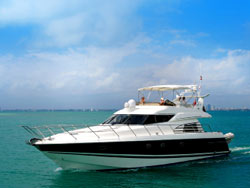
\includegraphics[width=\linewidth]{boat.jpg} %this sets the pic to the width of the page; {file path}
  		\caption{A boat.}    %this is the caption that goes undernath the picture
  		\label{fig:boat1}   %this is not seen on the document but is useful for referring to the picture 
	\end{figure}

	Figure \ref{fig:boat1} shows a boat. %the ref part will give 1 in this case
	
	%forcing a picture to a certain position - force the float
	%h  - same location
	%t - top of page
	%b - bottom of page
	%p - on an extra page
	%! - will force teh specified location
	%to force in same location do  \begin{figure} [h!]

	%need to compile TWO times for contents etc.

    
\end{document}